\documentclass[12pt,a4paper]{article}
\usepackage[indonesian]{babel}
\usepackage{times}
\usepackage{microtype}

\usepackage[top=4cm, left=4cm, right=3cm, bottom=3cm]{geometry}

\usepackage{setspace}
\usepackage{graphicx}
\usepackage{float}
\onehalfspacing

\setlength{\parindent}{1cm}

\begin{document}

\begin{titlepage}
  \begin{center}
    \singlespacing

    {\Large\bfseries MAKALAH INFRASTUKTUR FTTH:}\\[0.3cm]
    {\Large\bfseries DALAM PERUSAHAAN MYREPUBLIC}\\[0.3cm]

    % Logo Makalah
    \vspace{2cm}
    
\includegraphics[width=8cm]{images.jpeg}\\[2cm]

    {\large\bfseries Disusun oleh:}\\[0.3cm]
    {\large 
      Maulana Yusuf Apriliansyah $_1$\\
      Wisam Yassar Mahardika $_2$\\
      Ricky Juliana Sodikin $_3$\\
      Aliif Abdu Mukhti Al-Ghifari $_4$\\
      Devant Fadhillah $_5$\\
      Rafli Saeful Rukmana $_6$ \\[2cm]
    }

    {\large\bfseries SMK PLUS PRATAMA ADI}\\
    {\large\bfseries KOTA BANDUNG}\\
    {\large\bfseries 2026}

  \end{center}
\end{titlepage}

\newpage

\tableofcontents

\newpage

\section{Pendahuluan}

Perkembangan teknologi informasi dan komunikasi di era digital saat ini menuntut tersedianya layanan internet yang tidak hanya cepat, tetapi juga stabil dan dapat diandalkan. Kehadiran teknologi fiber optik telah merevolusi cara data ditransmisikan, menggantikan infrastruktur kabel tembaga tradisional yang memiliki banyak keterbatasan dalam hal kecepatan dan redaman jarak. Salah satu implementasi teknologi fiber optik yang paling masif digunakan untuk melayani pengguna rumahan adalah \textit{Fiber to the Home} (FTTH).

Makalah ini bertujuan untuk mengupas tuntas arsitektur dan infrastruktur FTTH, dengan mengambil studi kasus pada salah satu Penyedia Jasa Internet (ISP) terkemuka di Indonesia, yaitu MyRepublic. Melalui makalah ini, akan dibahas mulai dari profil perusahaan, target pelanggan, prinsip kerja FTTH, desain topologi jaringan, perangkat keras yang digunakan, perencanaan kapasitas, hingga penanganan gangguan yang sering terjadi di lapangan.

\section{Profil Perusahaan}

MyRepublic adalah perusahaan penyedia layanan internet (ISP) multinasional yang awalnya didirikan di Singapura pada tahun 2011. Di Indonesia, MyRepublic beroperasi di bawah naungan PT Innovate Mas Indonesia dan Grup Sinarmas, serta resmi meluncurkan layanannya pada tahun 2015. 

Identitas penyedia layanan ini sangat lekat dengan citra internet super cepat yang dikhususkan untuk kebutuhan hiburan tingkat tinggi, seperti \textit{gaming}, \textit{streaming} video beresolusi tinggi, dan \textit{unduhan} berkas besar. MyRepublic mengusung slogan ``Pride to be your pride'' dan sering kali menggunakan penekanan pada frasa \textit{``Streaming, Gaming, Surfing tanpa batas''}. Logo perusahaan didominasi oleh warna ungu khas yang melambangkan inovasi, kecepatan, dan teknologi masa depan yang premium. Fokus utama MyRepublic adalah memberikan pengalaman latensi rendah (\textit{low latency}) dengan rasio pengunduhan dan pengunggahan yang simetris atau mendekati simetris, menjadikannya salah satu pilihan favorit para \textit{gamer} dan pembuat konten di Indonesia.

\begin{figure}[H]
    \centering
    
\includegraphics[width=0.8\textwidth]{logo_my_republic.png}
    \caption{Logo MyRepublic}
    \label{fig:logo_myrepublic}
\end{figure}


\section{Target Pelanggan}

Target pelanggan MyRepublic diklasifikasikan ke dalam beberapa segmen utama dengan fokus pada kebutuhan konsumsi \textit{bandwidth} besar:

\begin{enumerate}
    \item \textbf{Kawasan Perumahan dan Apartemen (\textit{Residential}):} Menargetkan keluarga modern yang membutuhkan akses internet multi-perangkat untuk \textit{smart home}, \textit{streaming} Netflix/YouTube di Smart TV, dan sekolah daring. Area yang dijangkau difokuskan pada pemukiman padat dan terencana di kawasan sub-urban dan urban.
    \item \textbf{Penggiat E-Sports dan \textit{Gamer}:} MyRepublic mendesain \textit{routing} jaringan khusus yang dioptimalkan untuk mengurangi latensi (\textit{ping}) ke berbagai peladen (\textit{server}) gim internasional, sehingga sangat diminati oleh pemain gim daring kompetitif.
    \item \textbf{Usaha Mikro, Kecil, dan Menengah (UMKM):} Selain perumahan, penyedia layanan ini juga menyediakan paket bisnis berskala kecil seperti kedai kopi, kantor \textit{startup}, atau ruko yang memerlukan koneksi andal untuk operasional harian.
    \item \textbf{Lingkungan Pendidikan:} Beberapa wilayah kampus dan sekolah menengah juga menjadi target perluasan jaringan untuk menunjang kegiatan laboratorium komputer dan administrasi berbasis web.
\end{enumerate}

\section{Pengenalan FTTH}

\textit{Fiber to the Home} (FTTH) adalah suatu format penghantaran sinyal optik dari pusat penyedia layanan (Sentral/STO) langsung ke rumah-rumah pelanggan menggunakan media kabel serat optik. Pada teknologi ini, data dalam bentuk sinyal elektrik diubah menjadi sinyal cahaya (foton) menggunakan laser. Cahaya ini kemudian merambat di dalam serat kaca tipis berskala mikrometer.

Keunggulan utama FTTH dibandingkan kabel tembaga (seperti ADSL) adalah kemampuannya membawa \textit{bandwidth} hingga skala Gigabit per detik (Gbps), bebas dari interferensi gelombang elektromagnetik, serta redaman sinyal yang sangat kecil meski ditarik hingga jarak 20 kilometer dari sentral. Pada sistem yang digunakan MyRepublic, teknologi yang umum diterapkan adalah GPON (\textit{Gigabit Passive Optical Network}), di mana pemisahan kabel menuju banyak rumah pelanggan tidak menggunakan perangkat bertenaga listrik, melainkan prisma pemecah cahaya (\textit{passive splitter}).

\begin{figure}[H]
    \centering
    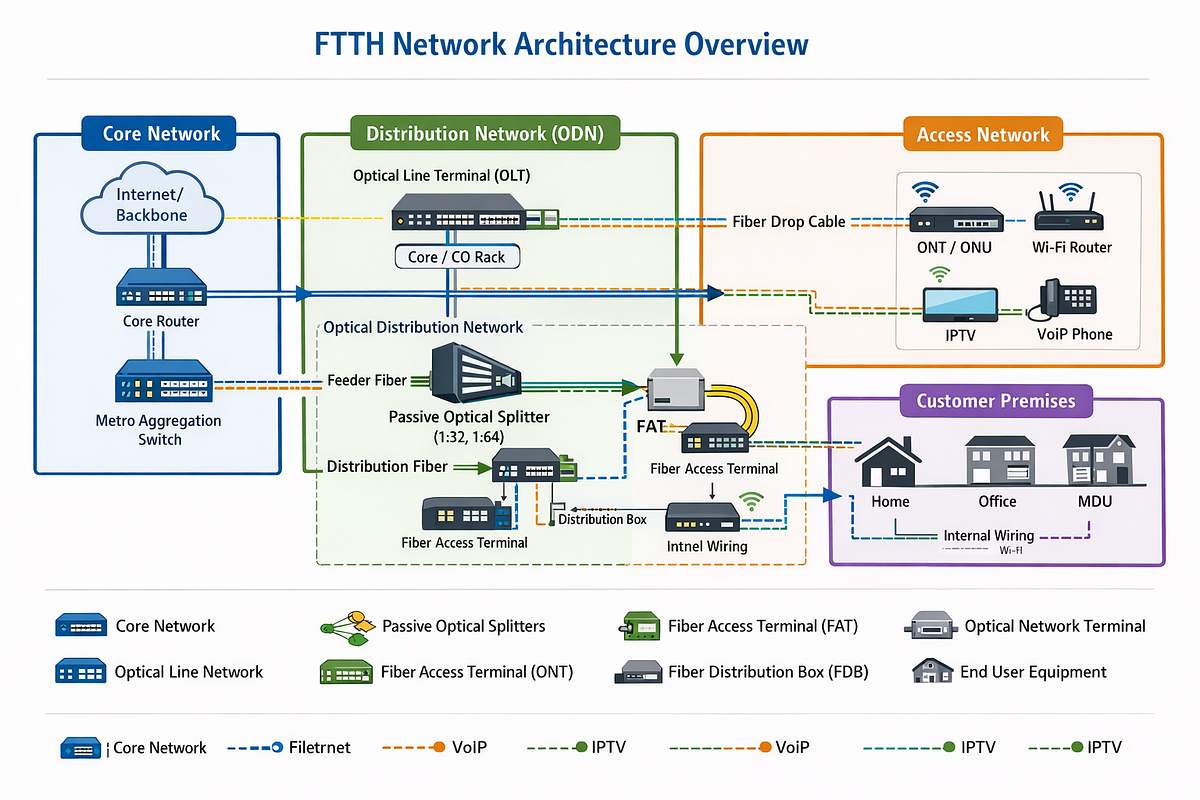
\includegraphics[width=0.8\textwidth]{ilustrasi_ftth.png}
    \caption{Skema Dasar Konsep Fiber to the Home (FTTH)}
    \label{fig:ftth_intro}
\end{figure}

\section{Desain Topologi}

Jaringan FTTH MyRepublic membentang dari pusat data (Headend/Sentral) hingga ke perangkat di ruang tamu pelanggan. Alur jaringan topologinya disusun secara hierarkis:

\begin{itemize}
    \item \textbf{Sentral ISP (Headend):} Lokasi di mana perangkat OLT (\textit{Optical Line Terminal}) berada dan terhubung ke \textit{router} distribusi utama.
    \item \textbf{Kabel Feeder (Kabel Utama):} Kabel optik berkapasitas besar (biasanya berisi puluhan hingga ratusan \textit{core}) ditarik dari OLT menuju titik kumpul suatu wilayah.
    \item \textbf{ODC (\textit{Optical Distribution Cabinet}):} Lemari di pinggir jalan tempat memecah 1 kabel \textit{feeder} menjadi beberapa kabel distribusi menggunakan komponen \textit{splitter} pasif tahap pertama (misal rasio 1:4).
    \item \textbf{Kabel Distribusi:} Kabel yang ditarik dari ODC menuju tiang-tiang di kompleks perumahan pelanggan.
    \item \textbf{ODP (\textit{Optical Distribution Point}):} Kotak kecil di tiang (atau bawah tanah) yang berisi \textit{splitter} tahap kedua (misal rasio 1:8). Dari sini kabel akan ditarik ke rumah-rumah.
    \item \textbf{Kabel Drop (\textit{Drop Wire}):} Kabel optik pelindung tebal berisi 1 atau 2 \textit{core} yang ditarik dari tiang ODP menuju atap rumah pelanggan.
    \item \textbf{Roset dan Patchcord:} Titik terminasi di dinding rumah pelanggan, disambung kabel kuning pendek (\textit{patchcord}) menuju modem.
    \item \textbf{ONT (\textit{Optical Network Terminal}):} Titik akhir topologi, perangkat yang mengubah kembali cahaya menjadi koneksi \textit{Ethernet/Wi-Fi} untuk gawai pengguna.
\end{itemize}

\begin{figure}[H]
    \centering
    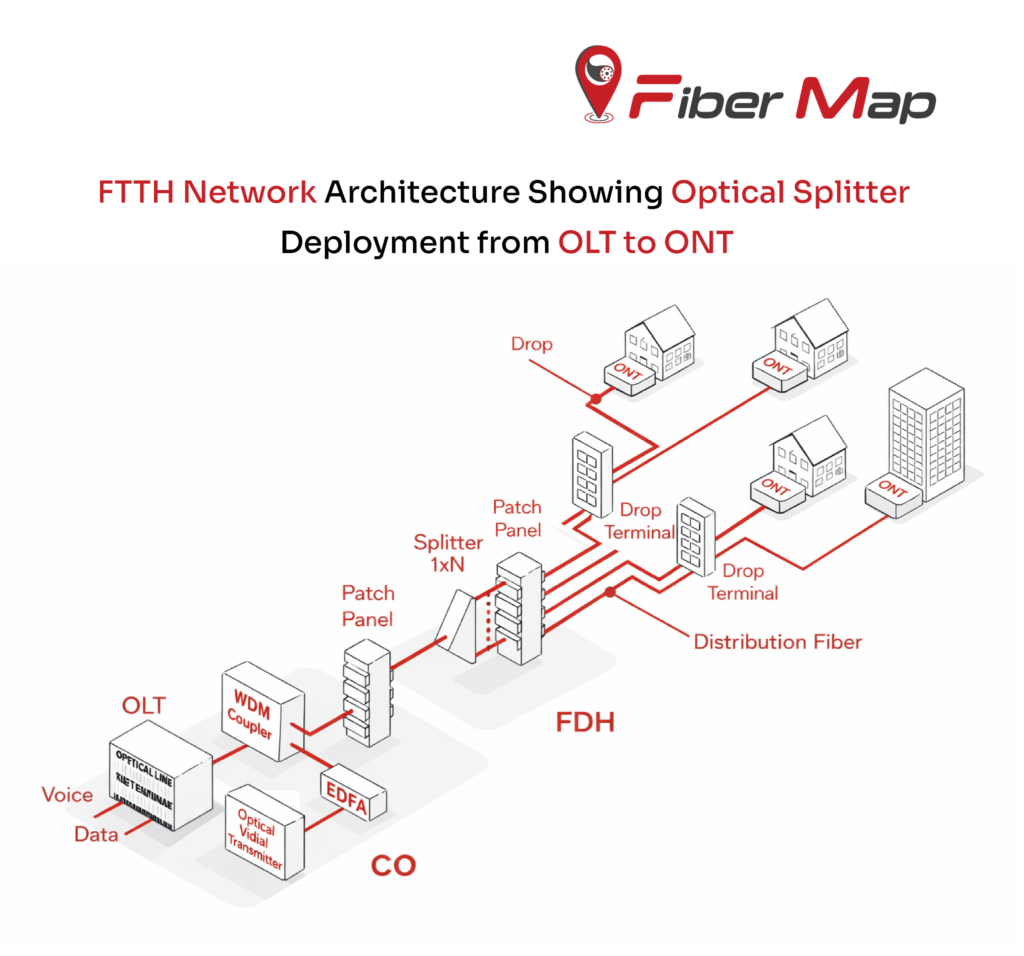
\includegraphics[width=0.9\textwidth]{topologi_jaringan.png}
    \caption{Desain Topologi FTTH GPON}
    \label{fig:topologi}
\end{figure}

\section{Perangkat Jaringan}

Infrastruktur FTTH dibentuk oleh serangkaian perangkat aktif (membutuhkan listrik) dan pasif (tidak membutuhkan listrik).

\begin{enumerate}
    \item \textbf{OLT (\textit{Optical Line Terminal}):} Perangkat aktif sentral penyedia. Berfungsi sebagai antarmuka antara sistem jaringan \textit{backbone} MyRepublic dengan jaringan akses GPON. OLT mengatur pengiriman dan penerimaan sinyal secara multipleks ke ribuan pelanggan sekaligus.
    \item \textbf{Kabel Fiber Optik:} Media transmisi berbasis serat kaca utuh. Terbagi menjadi kabel \textit{feeder} (jalur utama), kabel distribusi (jalur cabang perumahan), dan kabel \textit{drop} (jalur akses ke rumah).
    \item \textbf{ODC (\textit{Optical Distribution Cabinet}):} Lemari terminal pasif yang melindungi sambungan (\textit{splicing}) antara kabel \textit{feeder} dan kabel distribusi.
    \item \textbf{Optical Splitter:} Prisma kaca pasif yang membelah satu sorotan cahaya menjadi beberapa cabang (contoh: 1:4, 1:8, atau 1:16) tanpa memori atau suplai daya.
    \item \textbf{ODP (\textit{Optical Distribution Point}):} Kotak penutup pasif (umumnya hitam/abu-abu menempel pada tiang listrik/telkom) yang memfasilitasi terminasi kabel distribusi ke kabel \textit{drop} pelanggan.
    \item \textbf{ONT (\textit{Optical Network Terminal}):} Perangkat aktif pelanggan (sering disebut modem). Mengubah sinyal optik kembali menjadi sinyal elektrik (kabel LAN RJ45) dan gelombang nirkabel (Wi-Fi 2.4GHz / 5GHz) serta mendistribusikan IP lokal di rumah pelanggan.
\end{enumerate}

\section{Perencanaan Kapasitas}

Dalam membangun jaringan FTTH di sebuah kawasan perumahan, MyRepublic sebagai ISP harus melakukan perencanaan dan simulasi matang agar sumber daya efisien namun siap menampung seluruh rumah. 

Misalkan kita melakukan simulasi pada sebuah kompleks ``Perumahan Pratama Alam'' yang berkapasitas 100 rumah. Jika ISP menargetkan penetrasi 80\% (target 80 pelanggan di masa depan):

\begin{itemize}
    \item \textbf{Kebutuhan ODP:} ODP standar umumnya memiliki rasio \textit{splitter} 1:8 (melayani maksimal 8 rumah). Untuk 80 pelanggan, dibutuhkan minimal 10 buah ODP yang tersebar di tiang-tiang perumahan tersebut.
    \item \textbf{Kebutuhan ODC:} 10 buah ODP ini akan ditarik menuju 1 titik ODC terdekat di luar kompleks.
    \item \textbf{Pemakaian Splitter:} Di dalam ODC, kabel dari OLT dipasang pada \textit{splitter} 1:16. Artinya, 1 urat kabel optik inti (1 \textit{core}) dari Sentral MyRepublic yang masuk ke ODC dapat dipecah menjadi 16 jalur, di mana 10 jalur akan digunakan untuk memakan 10 kotak ODP di perumahan tersebut (sisa 6 jalur sebagai cadangan atau ekspansi perumahan sebelah).
    \item \textbf{Kebutuhan Port OLT:} Teknologi GPON rata-rata mendukung total pemecahan hingga 1:64 atau 1:128 per satu antarmuka (Port PON) di sentral. Oleh karena itu, seluruh kompleks Perumahan Pratama Alam (100 rumah) hanya akan memakai kapasitas 1 Port PON pada sasis OLT MyRepublic.
    \item \textbf{Kabel Fiber:} Diperlukan sekitar 1--2 km kabel distribusi (\textit{24/48 core}) menyusuri jalan kompleks, dan sekumpulan gulungan kabel \textit{drop} sepanjang 50--150 meter per titik pelanggan ketika dilakukan instalasi.
\end{itemize}

\section{Paket Layanan}

Sebagai penyedia layanan internet yang fokus pada hiburan dan kecepatan tinggi, MyRepublic menawarkan ragam pilihan langganan. Berikut adalah contoh 3 paket utama yang populer di kalangan pelanggan \textit{residential}:

\begin{enumerate}
    \item \textbf{Paket Value (Up to 30 Mbps - 50 Mbps):}\\
    Paket \textit{entry-level} ini ditujukan bagi rumah tangga berukuran kecil hingga menengah. Cocok untuk menelusuri web ringan, media sosial, dan \textit{streaming} video beresolusi 1080p dengan batas jumlah gawai terhubung 3 hingga 5 unit.
    \item \textbf{Paket Fast (Up to 100 Mbps - 150 Mbps):}\\
    Merupakan paket standar untuk keluarga modern dengan pemakaian \textit{bandwidth} berat harian. Sangat mendukung resolusi \textit{streaming} 4K (Ultra HD), pembelajaran jarak jauh, konferensi video multipengguna tanpa terputus, dan kecepatan unduhan berkas yang andal.
    \item \textbf{Paket MyGamer (Up to 250 Mbps - 500 Mbps):}\\
    Paket \textit{flagship} MyRepublic yang dirancang eksklusif. Dilengkapi dengan jalur khusus (\textit{custom routing}), dan alamat IP Publik Statis untuk menjaga latensi tetap sangat rendah bagi gim kompetitif di konsol maupun PC, serta memiliki proporsi kecepatan unggah ganda (\textit{symmetrical upload/download}) untuk \textit{live streaming} gim.
\end{enumerate}

\begin{figure}[H]
    \centering
    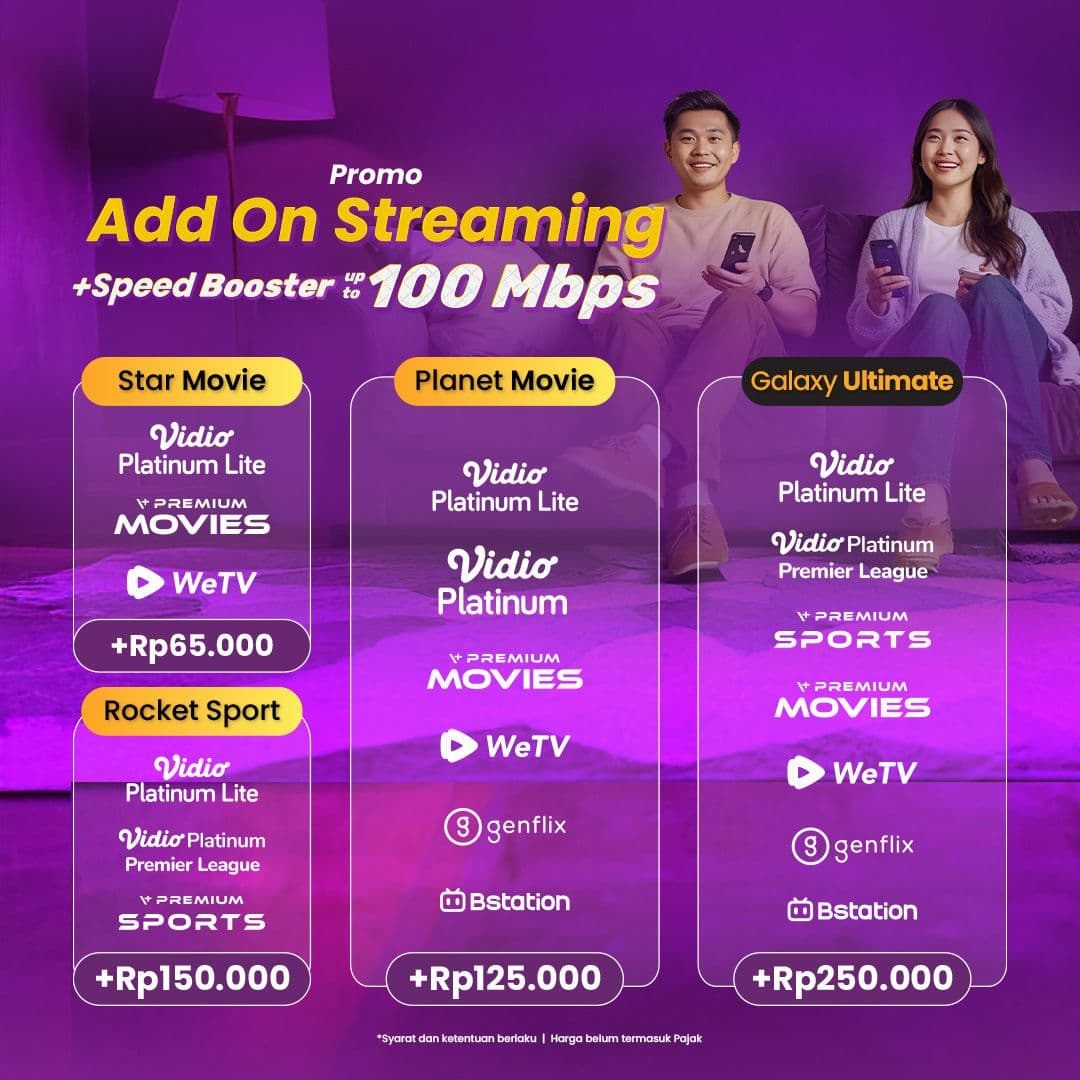
\includegraphics[width=0.31\textwidth]{paket_layanan_1.jpeg}\hfill
    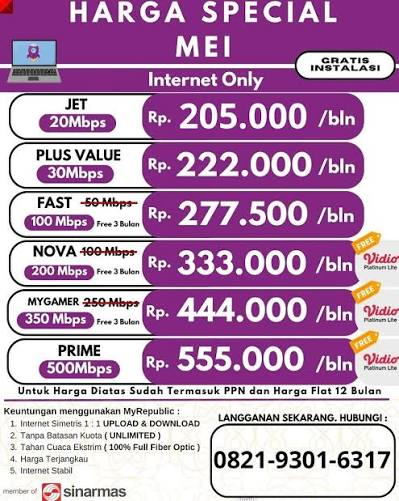
\includegraphics[width=0.31\textwidth]{paket_layanan_2.jpeg}\hfill
    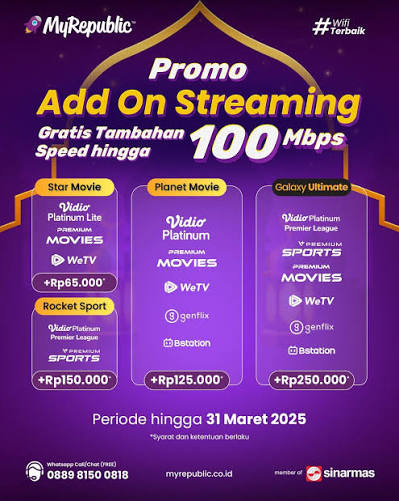
\includegraphics[width=0.31\textwidth]{paket_layanan_3.jpeg}
    \caption{Visualisasi Paket Layanan Internet MyRepublic}
    \label{fig:paket}
\end{figure}

\section{Gangguan Jaringan}

Meski berbasis serat optik yang stabil, infrastruktur fisik FTTH rentan terhadap gangguan. Berikut adalah tiga kasus insiden utama beserta penanganan teknisnya:

\begin{enumerate}
    \item \textbf{Kabel Drop Terputus (Red LOS):}\\
    \textit{Gangguan:} Lampu indikator `LOS' berkedip merah pada modem (ONT). Sering terjadi akibat kabel fiber pelanggan tergigit tikus, tertimpa dahan pohon layu, atau tersangkut kendaraan melintas di luar rumah.\\
    \textit{Solusi Teknis:} Teknisi lapangan harus datang, mencari titik putus visual, dan melakukan penyambungan optik ulang menggunakan alat \textit{Splicer} (Fusion Splicer) atau bahkan mengganti satu gulung rute kabel drop jika kerusakannya berat.
    \item \textbf{Redaman Sinyal Tinggi (\textit{High Attenuation}):}\\
    \textit{Gangguan:} Internet sering \textit{putus-nyambung} (\textit{intermittent}) dan lambat meski indikator LOS mati, lampu PON berkedip perlahan. Umumnya terjadi akibat tekukan tajam (\textit{bending loss}) pada ujung konektor atau debu yang masuk ke lubang roset.\\
    \textit{Solusi Teknis:} Mengecek rasio desibel (dBm) cahaya dengan \textit{Optical Power Meter} (OPM). Teknisi akan merapikan kabel yang tertekuk dan membersihkan jarum konektor UPC/APC memakai \textit{fiber cleaner} khusus berbahan alkohol 99\%.
    \item \textbf{Modem (ONT) Rusak Terkena Lonjakan Listrik:}\\
    \textit{Gangguan:} Saat wilayah sekitar sedang ada perbaikan tiang listrik atau petir, ONT pelanggan mati total dan tidak mengeluarkan pancaran sinyal Wi-Fi, karena adaptor daya terbakar.\\
    \textit{Solusi Teknis:} Proses pendaftaran (\textit{registration}) ulang perangkat keras baru. Teknisi mengganti \textit{adaptor} atau keseluruhan ONT. \textit{Serial Number} (SN) dari modem baru tersebut lalu diregistrasi kembali pada sistem OLT dari pusat MyRepublic agar kembali mendapat sinkronisasi profil IP.
\end{enumerate}

\section{Penutup}

Infrastruktur FTTH telah menjadi tulang punggung revolusi konektivitas era modern. Arsitektur jaringan dari sentral ISP menuju rumah dengan teknologi komponen GPON menjamin penghantaran data berskala raksasa, bebas karat, dan latensi mini. Implementasi ekosistem optik tersebut dijalankan secara profesional oleh MyRepublic di Indonesia. 

Dengan menyasar pasar yang spesifik—seperti \textit{gamer} kompetitif dan kawasan perumahan intensif \textit{streaming}—MyRepublic telah mendesain perencanaan kapasitas melalui titik distribusi pasif (ODP dan ODC) secara efisien di lapangan. Gangguan pada komponen fisik serat optik (seperti degradasi akibat debu maupun putusnya kabel \textit{drop}) dapat diminimalisir dan ditangani oleh tim penyambung lapangan menggunakan pedoman standar yang terukur. Pada akhirnya, inovasi tiada henti pada media jaringan transmisi FTTH ini menjamin pengalaman dunia digital pelanggan rumahan terfasilitasi dengan sempurna di masa depan.

\newpage

\begin{thebibliography}{99}
    \bibitem{apjii2020} Asosiasi Penyelenggara Jasa Internet Indonesia (APJII). (2020). \textit{Laporan Survei Penetrasi dan Profil Perilaku Pengguna Internet Indonesia}. APJII.
    \bibitem{tanenbaum2011} Tanenbaum, A. S., \& Wetherall, D. J. (2011). \textit{Computer Networks} (5th ed.). Pearson Education.
    \bibitem{itu_gpon} International Telecommunication Union (ITU-T). (2008). \textit{G.984 Series: Gigabit-capable passive optical networks (GPON)}. ITU Publications.
    \bibitem{myrep_web} MyRepublic Indonesia. (2023). \textit{Layanan Internet dan Profil Perusahaan}. Diakses dari website resmi MyRepublic.
    \bibitem{fiber2015} Keiser, Gerd. (2015). \textit{Optical Fiber Communications} (5th ed.). McGraw-Hill Education.
\end{thebibliography}

\end{document}
